\begin{topic}{quantized-universal-enveloping-algebra}{quantized universal enveloping algebra}
    Let $\mathfrak{g}$ be a complex \tref{simple-lie-algebra}{semisimple Lie algebra}, $\Pi = \{ \alpha_1, \ldots, \alpha_n \}$ a set of \tref{root-system-lie-algebra}{simple roots} for $\mathfrak{g}$, and $A = (a_{ij})$ the corresponding \tref{LA:cartan-matrix}{Cartan matrix}. For any $q \in \CC^*$, the \textbf{quantized universal enveloping algebra} $U_q(\mathfrak{g})$ is the complex algebra generated by $E_i, F_i, K_i, K_i^{-1}$, with $1 \le i \le n$, satisfying the relations
    \[ K_i K_i^{-1} = K_i^{-1} K_i = 1, \quad K_i K_j = K_j K_i , \]
    \[ K_i E_j K_i^{-1} = q_{i}^{a_{i j}} E_j, \quad K_i F_j K_i^{-1} = q_{i}^{-a_{i j}} F_j , \]
    \[ E_i F_j - F_j E_i = \delta_{i j} \frac{K_i - K_i^{-1}}{q_i - q_i^{-1}} , \]
    with $q_i = q^{\frac{1}{2} (\alpha_i, \alpha_i)}$, and for $i \ne j$ the \textit{quantum Serre relations}
    \[ \begin{aligned}
        \sum_{k = 0}^{1 - a_{i j}} (-1)^k \binom{1 - a_{i j}}{k}_{q_i} E_i^{1 - a_{i j} - k} E_j E_i^k &= 0 , \\
        \sum_{k = 0}^{1 - a_{i j}} (-1)^k \binom{1 - a_{i j}}{k}_{q_i} F_i^{1 - a_{i j} - k} F_j F_i^k &= 0 ,
    \end{aligned} \]
    where $\binom{m}{n}_q = \frac{[m]_q!}{[n]_q! [m - n]_q!}$ denotes the \textit{quantum binomial}, and $[m]_q! = \prod_{k = 1}^{m} \frac{q^k - q^{-k}}{q - q^{-1}}$ the \textit{quantum factorial}.
\end{topic}

\begin{example}{quantized-universal-enveloping-algebra}
    For $\mathfrak{g} = \mathfrak{sl}_2(\CC)$, the quantized universal enveloping algebra $U_q(\mathfrak{sl}_2(\CC))$ is generated by $E, F, K^{\pm 1}$ and subject to the relations
    \[ KK^{-1} = K^{-1} K = 1, \quad KEK^{-1} = q^2 E, \quad KFK^{-1} = q^{-2} F, \quad EF - FE = \frac{K - K^{-1}}{q - q^{-1}} . \]
\end{example}

\begin{example}{quantized-universal-enveloping-algebra}
    The quantized algebra $U_q(\mathfrak{g})$ naturally has the structure of a \tref{hopf-algebra}{Hopf algebra}, given by
    \[ \Delta(K_i) = K_i \otimes K_i, \quad \Delta(E_i) = E_i \otimes 1 + K_i \otimes E_i, \quad \Delta(F_i) = F_i \otimes K_i^{-1} + 1 \otimes F_i , \]
    \[ \varepsilon(K_i) = 1, \quad \varepsilon(E_i) = 0, \quad \varepsilon(F_i) = 0 , \]
    \[ S(K_i) = K_i^{-1}, \quad S(E_i) = -K_i^{-1} E_i, \quad S(F_i) = - F_i K_i . \]
\end{example}

\begin{topic}{universal-r-matrix}{universal R-matrix}
    Let $A$ be a \tref{hopf-algebra}{Hopf algebra} with comultiplication $\Delta$. An invertible element $R \in A \otimes A$ is called a \textbf{universal $R$-matrix} for $A$ if it satisfies
    \[ (\Delta \otimes \id) R = R_{13} R_{23}, \quad (\id \otimes \Delta) R = R_{13} R_{12}, \quad \tau \circ \Delta (a) = R \Delta(a) R^{-1} \textup{ for all } a \in A , \]
    where $\tau : A \otimes A \to A \otimes A$ is the flip map $\tau(a \otimes b) = b \otimes a$, and furthermore $R = \sum_i a_i \otimes b_i$, $R_{12} = \sum_i a_i \otimes b_i \otimes 1$, $R_{13} = \sum_i a_i \otimes 1 \otimes b_i$ and $R_{23} = \sum_i 1 \otimes a_i \otimes b_i$.
\end{topic}

\begin{example}{universal-r-matrix}
    \textit{Sweedler's Hopf algebra} is the Hopf algebra $A$ generated by two elements $x$ and $y$ and relations
    \[ x^2 = 1, \quad y^2 = 0, \quad xy + yx = 0 , \]
    whose Hopf algebra structure given by
    \[ \Delta(x) = x \otimes x, \quad \Delta(y) = 1 \otimes y + y \otimes x, \quad S(x) = x, \quad S(y) = xy, \quad \varepsilon(x) = 1, \quad \varepsilon(y) = 0 . \]
    For any $q \in k$, the matrix
    \[ R_q = \frac{1}{2} (1 \otimes 1 + 1 \otimes x + x \otimes 1 - x \otimes x) + \frac{q}{2} (y \otimes y + y \otimes xy + xy \otimes xy - xy \otimes y) \]
    is a universal $R$-matrix for $A$. Note that $R_q^{-1} = \tau_{A, A}(R_q)$.
\end{example}

\begin{example}{universal-r-matrix}
    Any universal $R$-matrix $R$ of $A$ satisfies the \tref{quantum-yang-baxter-equation}{quantum Yang--Baxter equation}, as
    \[ \begin{aligned}
        R_{12} R_{13} R_{23}
            &= R_{12} (\Delta \otimes \id) R \\
            &= ((\tau_{A, A} \circ \Delta \otimes \id) R) R_{12} \\ 
            &= ((\tau_{A, A} \otimes \id)(\Delta \otimes \id) R) R_{12} \\
            &= ((\tau_{A, A} \otimes \id) R_{13} R_{23}) R_{12} \\
            &= R_{23} R_{13} R_{12} . 
    \end{aligned} \]
\end{example}

\begin{example}{universal-r-matrix}
    Let $A$ be a Hopf algebra over a field $k$, and consider the \tref{CT:monoidal-category}{monoidal category} of (left) $A$-modules. The tensor product of $A$-modules $V$ and $W$ is given by $V \otimes_k W$, where $a \cdot (v \otimes w) = \Delta(a) \cdot (v, w)$, and the unit is the one-dimensional vector space $\textbf{1} = k$ with $a \cdot \lambda = \varepsilon(a) \lambda$. This being a monoidal category follows from $A$ being a \tref{bialgebra}{bialgebra}.
    
    Now a universal $R$-matrix $R$ precisely corresponds to a \tref{CT:braided-monoidal-category}{braiding}
    \[ c_{V, W}^R(v \otimes w) = \tau_{V, W}(R (v \otimes w)) . \]
    Conversely, from a braiding $c$ one can obtain a universal $R$-matrix as
    \[ R = \tau_{A, A}(c_{A, A}(1 \otimes 1)) . \]
\end{example}

\begin{topic}{quantum-yang-baxter-equation}{quantum Yang--Baxter equation}
    Let $V$ be a \tref{LA:vector-space}{vector space}, and $R : V \otimes V \to V \otimes V$ an endomorphism. Writing $R = \sum_i a_i \otimes b_i$, the \textbf{quantum Yang--Baxter equation} is the equation
    \[ R_{23} R_{13} R_{12} = R_{12} R_{13} R_{23} , \]
    where
    \[ R_{12} = \sum_i a_i \otimes b_i \otimes 1, \quad R_{13} = \sum_i a_i \otimes 1 \otimes b_i, \quad R_{23} = \sum_i 1 \otimes a_i \otimes b_i . \]
\end{topic}

\begin{example}{quantum-yang-baxter-equation}
    Consider a physical quantum system consisting of three identical particles, each modeled by a vector space $V$. The interaction of two colliding particles can be represented by an endomorphism $R : V \otimes V \to V \otimes V$. From relativistic principles, the order of interactions should not matter, so the following diagrams should correspond to the same interaction.
    \[ 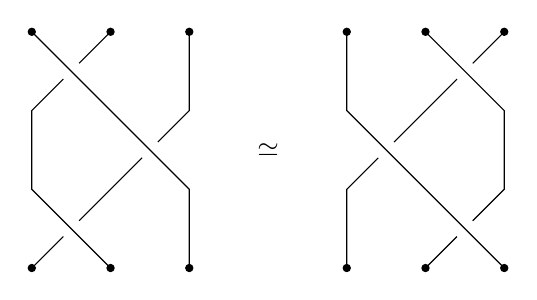
\begin{tikzpicture}
        \begin{scope}
            \draw[black,fill=black] (0, 0) circle (.3ex);
            \draw[black,fill=black] (1, 0) circle (.3ex);
            \draw[black,fill=black] (2, 0) circle (.3ex);
            \draw[black,fill=black] (0, 3) circle (.3ex);
            \draw[black,fill=black] (1, 3) circle (.3ex);
            \draw[black,fill=black] (2, 3) circle (.3ex);
            \draw (0, 3) -- (1, 2) -- (2, 1) -- (2, 0);
            \draw (1, 3) -- (0.6, 2.6);
            \draw (0.4, 2.4) -- (0, 2) -- (0, 1) -- (1, 0);
            \draw (2, 3) -- (2, 2) -- (1.6, 1.6);
            \draw (1.4, 1.4) -- (0.6, 0.6);
            \draw (0.4, 0.4) -- (0, 0);
        \end{scope}
        \node at (3cm,1.5cm) {$\simeq$};
        \begin{scope}[xshift=4cm]
            \draw[black,fill=black] (0, 0) circle (.3ex);
            \draw[black,fill=black] (1, 0) circle (.3ex);
            \draw[black,fill=black] (2, 0) circle (.3ex);
            \draw[black,fill=black] (0, 3) circle (.3ex);
            \draw[black,fill=black] (1, 3) circle (.3ex);
            \draw[black,fill=black] (2, 3) circle (.3ex);
            \draw (0, 3) -- (0, 2) -- (1, 1) -- (2, 0);
            \draw (1, 3) -- (2, 2) -- (2, 1) -- (1.6, 0.6);
            \draw (1.4, 0.4) -- (1, 0);
            \draw (2, 3) -- (1.6, 2.6);
            \draw (1.4, 2.4) -- (0.6, 1.6);
            \draw (0.4, 1.4) -- (0, 1) -- (0, 0);
        \end{scope}
    \end{tikzpicture} \]
    This relation precisely corresponds to the quantum Yang--Baxter equation.
\end{example}
